\documentclass[border=4pt]{standalone}
\usepackage[T1]{fontenc}
\usepackage{lmodern}
\usepackage{amsmath}
\usepackage{xcolor}
\usepackage{tikz}
\usetikzlibrary{positioning,arrows.meta,fit,backgrounds,calc}

% palette
\definecolor{cCon}{HTML}{C0392B} % constraint
\definecolor{cProc}{HTML}{2E86C1} % procedure
\definecolor{cBel}{HTML}{7D8A99}  % belief/other
\definecolor{cBudget}{HTML}{27AE60}
\definecolor{cInk}{HTML}{232323}
\definecolor{cPanel}{HTML}{F4F5F7}
\definecolor{cRule}{HTML}{CBD2D9}

\begin{document}
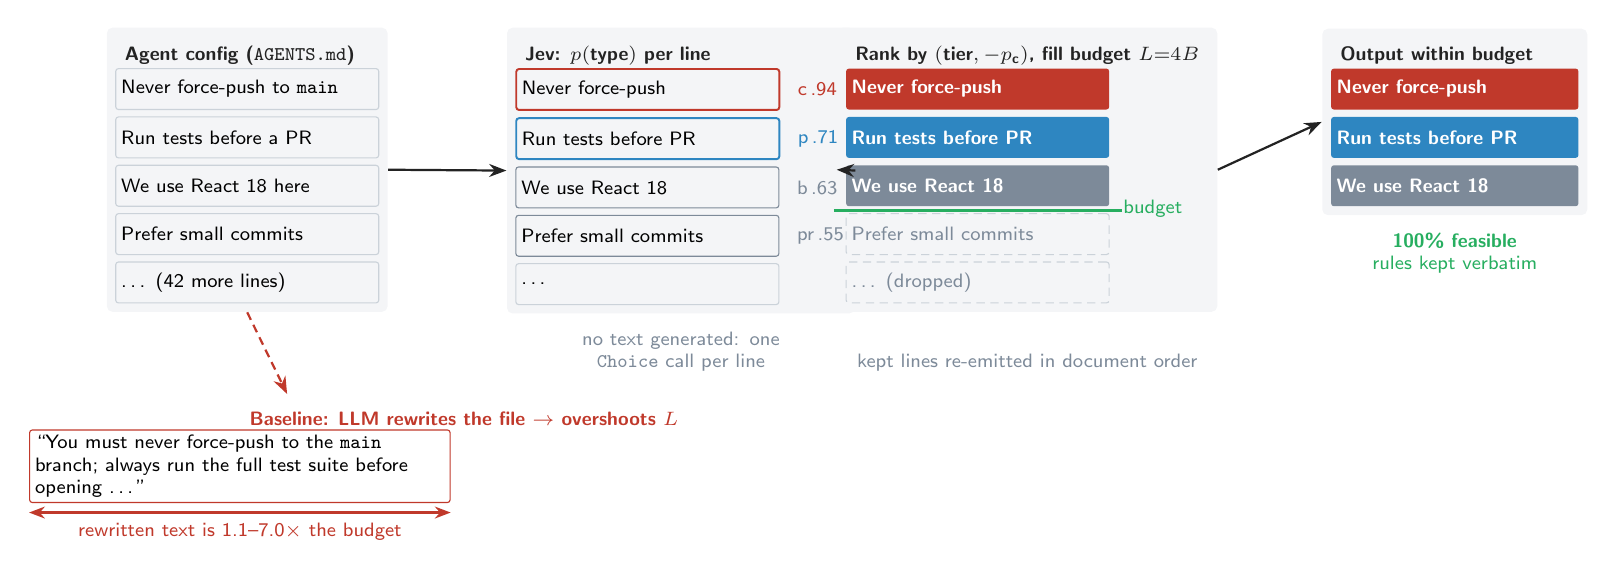
\begin{tikzpicture}[
  font=\sffamily\small,
  line/.style={-{Stealth[length=2.2mm]}, cInk, thick},
  lbl/.style={font=\sffamily\scriptsize\bfseries, cInk},
  capt/.style={font=\sffamily\scriptsize, cBel},
  row/.style={draw=cRule, rounded corners=1pt, minimum height=5.2mm, inner sep=2pt, font=\sffamily\scriptsize, anchor=west, text width=32mm},
  chip/.style={rounded corners=1pt, minimum height=5.2mm, inner sep=2pt, font=\sffamily\scriptsize\bfseries, text=white, anchor=west, text width=32mm},
  prob/.style={font=\sffamily\scriptsize, cBel, anchor=west},
]

% ---------- Stage 1: input config ----------
\node[lbl] (t1) at (0,0) {Agent config (\texttt{AGENTS.md})};
\node[row, below=1.6mm of t1.west, anchor=north west] (i1) {Never force-push to \texttt{main}};
\node[row, below=0.8mm of i1.south west, anchor=north west] (i2) {Run tests before a PR};
\node[row, below=0.8mm of i2.south west, anchor=north west] (i3) {We use React 18 here};
\node[row, below=0.8mm of i3.south west, anchor=north west] (i4) {Prefer small commits};
\node[row, below=0.8mm of i4.south west, anchor=north west] (i5) {\ldots\ (42 more lines)};
\begin{scope}[on background layer]
  \node[fill=cPanel, rounded corners=2pt, fit=(t1)(i1)(i5), inner sep=3pt] (box1) {};
\end{scope}

% ---------- Stage 2: Jev per-line probabilities ----------
\node[lbl] (t2) at (48mm,0) {Jev: $p(\text{type})$ per line};
\node[row, below=1.6mm of t2.west, anchor=north west, draw=cCon, line width=0.7pt] (j1)
  {Never force-push\hfill};
\node[prob, right=1mm of j1.east] (p1) {\textcolor{cCon}{c\,.94}};
\node[row, below=0.8mm of j1.south west, anchor=north west, draw=cProc, line width=0.7pt] (j2)
  {Run tests before PR\hfill};
\node[prob, right=1mm of j2.east] (p2) {\textcolor{cProc}{p\,.71}};
\node[row, below=0.8mm of j2.south west, anchor=north west, draw=cBel] (j3)
  {We use React 18\hfill};
\node[prob, right=1mm of j3.east] (p3) {\textcolor{cBel}{b\,.63}};
\node[row, below=0.8mm of j3.south west, anchor=north west, draw=cBel] (j4)
  {Prefer small commits\hfill};
\node[prob, right=1mm of j4.east] (p4) {\textcolor{cBel}{pr\,.55}};
\node[row, below=0.8mm of j4.south west, anchor=north west, draw=cRule] (j5)
  {\ldots\hfill};
\begin{scope}[on background layer]
  \node[fill=cPanel, rounded corners=2pt, fit=(t2)(j1)(p1)(j5), inner sep=3pt] (box2) {};
\end{scope}
\node[capt, below=1mm of box2.south, text width=42mm, align=center]
  {no text generated: one \texttt{Choice} call per line};

% ---------- Stage 3: rank + greedy budget fill ----------
\node[lbl] (t3) at (100mm,0) {Rank by $(\text{tier},-p_{\textsc{c}})$, fill budget $L{=}4B$};
\node[chip, fill=cCon, below=1.6mm of t3.west, anchor=north west] (r1) {Never force-push};
\node[chip, fill=cProc, below=0.8mm of r1.south west, anchor=north west] (r2) {Run tests before PR};
\node[chip, fill=cBel, below=0.8mm of r2.south west, anchor=north west] (r3) {We use React 18};
\node[row, below=0.8mm of r3.south west, anchor=north west, draw=cRule, densely dashed, text=cBel] (r4) {Prefer small commits};
\node[row, below=0.8mm of r4.south west, anchor=north west, draw=cRule, densely dashed, text=cBel] (r5) {\ldots\ (dropped)};
% budget bracket
\draw[cBudget, line width=1pt] ($(r3.south west)+(-1.5mm,-0.5mm)$) -- ($(r3.south east)+(1.5mm,-0.5mm)$);
\node[capt, text=cBudget, right=0.5mm of r3.south east, anchor=west, yshift=-0.3mm] {budget};
\begin{scope}[on background layer]
  \node[fill=cPanel, rounded corners=2pt, fit=(t3)(r1)(r5), inner sep=3pt] (box3) {};
\end{scope}
\node[capt, below=4mm of box3.south, text width=44mm, align=center]
  {kept lines re-emitted in document order};

% ---------- Stage 4: outputs comparison ----------
\node[lbl] (t4) at (152mm,0) {Output within budget};
\node[chip, fill=cCon, below=1.6mm of t4.west, anchor=north west, text width=30mm] (o1) {Never force-push};
\node[chip, fill=cProc, below=0.8mm of o1.south west, anchor=north west, text width=30mm] (o2) {Run tests before PR};
\node[chip, fill=cBel, below=0.8mm of o2.south west, anchor=north west, text width=30mm] (o3) {We use React 18};
\begin{scope}[on background layer]
  \node[fill=cPanel, rounded corners=2pt, fit=(t4)(o1)(o3), inner sep=3pt] (box4) {};
\end{scope}
\node[capt, below=1mm of box4.south, text width=32mm, align=center, text=cBudget]
  {\textbf{100\% feasible}\\rules kept verbatim};

% arrows between stages
\draw[line] (box1.east) -- (box2.west);
\draw[line] (box2.east) -- (box3.west);
\draw[line] (box3.east) -- (box4.west);

% ---------- contrast: LLM compaction overshoots ----------
\node[lbl, text=cCon, anchor=north west] (t5) at (0mm,-44mm) {Baseline: LLM rewrites the file $\rightarrow$ overshoots $L$};
\node[draw=cCon, rounded corners=1pt, minimum height=5mm, text width=52mm, inner sep=2pt,
      font=\sffamily\scriptsize, anchor=north west, below=1.4mm of t5.west] (llm)
  {``You must never force-push to the \texttt{main} branch; always run the full test suite before opening \ldots''};
\draw[cCon, line width=1pt, {Stealth[length=2mm]}-{Stealth[length=2mm]}]
  ($(llm.south west)+(0,-1.2mm)$) -- ($(llm.south east)+(0,-1.2mm)$)
  node[midway, below, font=\sffamily\scriptsize, text=cCon] {rewritten text is 1.1--7.0$\times$ the budget};
% connector from same input, branching down
\draw[line, cCon, densely dashed] (box1.south) -- ($(t5.north west)+(6mm,1mm)$);

\end{tikzpicture}
\end{document}
